\documentclass[12pt,a4paper]{report}

\usepackage{amsmath}
\usepackage{array}
\usepackage{float}

\usepackage{graphicx}
\graphicspath{{./images/}}

\usepackage{titlesec}
\titleformat{\chapter}[display]{\normalfont\scshape}{}{0pt}{\LARGE\flushright}[\tiny\HRule]
\titlespacing*{\chapter}{0pt}{-90pt}{10pt}

\usepackage{color}
\definecolor{javared}{rgb}{0.6,0,0} % for strings
\definecolor{javagreen}{rgb}{0.25,0.5,0.35} % comments
\definecolor{javapurple}{rgb}{0.5,0,0.35} % keywords
\definecolor{javadocblue}{rgb}{0.25,0.35,0.75} % javadoc

\usepackage{listings} 
\lstdefinestyle{eclipsejava}{language=Java,
basicstyle=\ttfamily\small,
keywordstyle=\color{javapurple}\bfseries,
stringstyle=\color{javared},
commentstyle=\color{javagreen},
morecomment=[s][\color{javadocblue}]{/**}{*/},
tabsize=2,
showspaces=false,
showstringspaces=false}
\lstset{style=eclipsejava}

%\renewcommand{\baselinestretch}{1.1}

\setlength{\parindent}{0pt}

\newcommand{\HRule}{\rule{\linewidth}{0.5mm}}

\newcommand{\zonejs}{zone.js}
\newcommand{\zonedrt}{dart:Zone}
\newcommand{\vertx}{Vert.x}


\begin{document}


\begin{titlepage}

  \newcommand{\rightside}[1]{
    \begin{flushright}
      \begin{minipage}[t]{0.48\textwidth}
        #1
      \end{minipage}
    \end{flushright}
  }


  \begin{center}
    
\includegraphics[height=0.1\textheight]{ELCA}
    \hfill
    
\includegraphics[height=0.1\textheight]{EPFL} \\[2cm]


    \rightside{
      \Large
      Master Thesis
      
      \small
      Distributed Programming Laboratory
    }


    \HRule
    \vspace{\baselineskip}

    \LARGE
    \textbf{
      % Control Flow Tracing through Asynchronous Context
      The Zone, a general model for asynchronous contexts
    }
    \normalsize
    \HRule
    
    \rightside{

      \vspace{1\baselineskip}

      \Large
      Val\'erian \textsc{Pittet}

      \vspace{2\baselineskip}

      \normalsize
      ELCA supervisors
      \smallskip
      \large
      \begin{list}{ }{}
      \item Philipp \textsc{Oser}
      \item Beno\^it \textsc{Briot}
      \end{list}
      
      \vspace{\baselineskip}

      \normalsize
      EPFL supervisor
      \smallskip
      \large
      \begin{list}{ }{}
      \item Rachid \textsc{Guerraoui}
      \end{list}


    }


    \vfill

    \normalsize
    August 14, 2015

  \end{center}

\end{titlepage}
\begin{abstract}

This research project targets the consistency concerns one meets when he write asynchronous programs. It offers overview and analysis of cases where our synchronous intuition (or \emph{mental model}) of program execution tricks us in assuming wrong hypothesis. It invites you to take some time to stop saying yourself ``I know how it works'' and try to explain yourself ``How does it work''.
In a sense, it tries to show the best answer to ``Why doesn't this code work ?'' may be ``Why did you think this would have worked ?''.
This allows to state clear limits on 
``What you want to do is simply impossible because it doesn't work that way. However the effect you want to archeive is possible, but require you to adapt your way of thinking to match the model you are using and not the model you \emph{think} you are using.''



\end{abstract}

\tableofcontents

\setlength{\parskip}{\baselineskip}


\chapter{Introduction}
\label{ch:intro}

Who never faced the challenge of debugging an asynchronous program? And even the somewhat simpler task of following its execution and understanding its dependencies is neither easy, as illustrated in chapter \ref{ch:motiv}.

The main reason of this difficulty is that our standard representations assume determinism and do not hold anymore with the non-determinism brought by the asynchrony.
However, this non-determinism is precisely what we search when using asynchronous constructs:~there is no way to bypass this problematic.

I propose a solution (chapter \ref{ch:zone}) inspired by the \zonejs\ and \zonedrt\ frameworks to implement functionalities that behave \emph{uniformly} in both synchronous and asynchronous contexts. Moreover this solution aims to be applicable to any underlying asynchronous implementation, at least the most common ones presented in chapter \ref{ch:asyncworld}. Chapter \ref{ch:approaches} shows how, unlike \zonejs\ and \zonedrt, the Zone for Java implements primitive features, allowing to compose almost any other functionality. This way, the Zone steps down central features as error handling or asynchronous execution tracing to a standard Zone plug-in. It also allows a great flexibility to add aspects fulfilling needs discovered later.

Practical experiments (chapter \ref{ch:inpractice}) built on top of the Zone showed how it supports modularization of complex properties, for example tracing each asynchronous transition of the program. On the other hand, integrating the Zone in an execution framework is hard (consider many cases, avoid duplicate binding), but this work must be done once. Then, use the instrumented executor and Zones will work transparently on any program based on that framework.

The Zone is an innovative tool in that it addresses the problem of implementing uniform behaviors across context modifications, regardless of the synchrony. The Zone allows you to think in terms of transitions between asynchronous tasks and simply implement those transitions once, at a single place.









% Initial objectives were very specific and usage targeted. Final implementation pushes those primary features to the level of optional ones that can be implemented using Zone primitives.



% This work presents my analysis and development process to build the final solution. A first pragmatic approach (Zone prototype) allowed me to grab and solve essential integration concerns :~How to represent the Zone and how to bind zoned code to it with minimal effort of the user.

% Then, naively adding properties implementing wished hooks/solution elements allowed me to quickly grasp the interest and power of the Zone, but also to face rough limitations preventing extension and composability of the Zone. As an answer to this, I developed a model (Zone model) that describes the core functions of the Zone which can be used to represent specific features. (Zone implementation)

% This model appears to be an innovative tool that drives you to think about asynchronous programs in a way you did not know before. We will see (Future work) potential extensions and refinements to both the model and the implementation to make the Zone an even more powerful and easy-to-use tool.



% \section{Objectives}

% \begin{itemize}
% \item Propose solution to stated problems
% \item Target the Java runtime environment
% \item Build an usable tool providing asynchronous execution context in a similar fashion to Zones in \zonejs\ and \zonedrt\.
% \item Targeted features include asynchronous error handling, long stack traces and generation of asynchronous sequence diagram.
% \item The tool should be easily usable and require few, if no adaptation in the user code. I will call this the integration concerns.
% \end{itemize}




\chapter{Motivations}
\label{ch:motiv}
To complete and give a clear idea of the problems I refer to, this chapter presents typical bugs encountered with asynchronous programming.

\section{Asynchronous Scope}

First problem with asynchronous execution is dealing with contextual values. Consider this simplistic code:

\begin{lstlisting}
Environment environment;

public void test() {
  environment = Environment.STANDARD;
  doStandardStuff();

  environment = Environment.CRITICAL;
  doCriticalStuff();

  environment = Environment.STANDARD;
  doStandardStuffAgain();
}
\end{lstlisting}

In synchronous code, there is no problem and everything runs with expected environment. Suppose now you need to improve performance. You change the method \lstinline{doCriticalStuff()} code to run asynchronously and forget to care about \lstinline{environment}. It's very likely that \lstinline{doCriticalStuff()} will run in a bad environment since it may execute \emph{after} \lstinline{environment} is modified.


This problem can be solved if we use a context persisting across asynchronous transitions to keep the environment value.


\section{Error Handling}

If the problem of asynchronous scope seems too basic to require attention, error handling already brings more challenge.

\begin{lstlisting}
public void test(int input) {
  
  try {
    heavyMathFunction(input);
  } catch (ArithmeticError e) {
    // handle error
  }

}
\end{lstlisting}

Again, as long as the code is synchronous there is no problem with the try-catch block. Once you decide to run asynchronously \lstinline{heavyMathFunction(int)} to avoid application freeze, the code may not handle (or even see) a runtime error.

A solution to this problem needs ways to keep error handler across asynchronous transitions or report asynchronous error to wrapping error handler.

\section{Error Tracing}

Suppose now asynchronous error are caught, debugging unexpected errors is still hard since the stack trace only goes back to the beginning of asynchronous execution. If the cause of the error precedes the asynchronous code submission, nothing can track it back.

\begin{lstlisting}
public void test() {

  int input1 = getInput1();
  startAsyncBatch(input1);
  // OK

  int input2 = getInput2();
  startAsyncBatch(input2);
  // OK

  int input3 = buggyGetInput();
  startAsyncBatch(input3);
  // bad implementation, gets bad input and throws
}
\end{lstlisting}

During execution, one error pops up, saying that the asynchronous batch got a bad input. It only indicates that somewhere in the code, \lstinline{startAsyncBatch(int)} was called with an invalid input. Imagine the stack trace going back before asynchronous execution. Finding the bug's origin is now a triviality. 

As illustration, consider this test code.

\begin{lstlisting}
private void pathStep1() {
  pathStep2();
}

private void pathStep2() {
  asyncExecutor1.execute(() -> pathStep3());
}

private void pathStep3() {
  pathStep4();
}

private void pathStep4() {
  asyncExecutor2.execute(() -> throw new TestError());
}
\end{lstlisting}

With standard stack traces, the error only indicates something like

\begin{lstlisting}
TestError: Unhandled intended testing error
        at Test.throwError(Test.java:102)
\end{lstlisting}

But using long stack traces produces

\begin{lstlisting}
TestError: Unhandled intended testing error
        at Test.throwError(Test.java:102)
           *****************************
           **        ASYNC GAP        **
           *****************************
        at Test.asyncThrow(Test.java:98)
        at Test.pathStep4(Test.java:94)
        at Test.pathStep3(Test.java:90)
           *****************************
           **        ASYNC GAP        **
           *****************************
        at Test.asyncExec(Test.java:86)
        at Test.pathStep2(Test.java:82)
        at Test.pathStep1(Test.java:78)
        at Test.test(Test.java:158)
\end{lstlisting}


To implement this, one could attribute a context value to each asynchronous execution containing the stack trace of the code that submitted the asynchronous code. Then on error handling, simply recover the asynchronous stack trace and add it to the caught error.

\section{Dependencies Tracking}

When asynchronous programs gets large, ordering and dependencies among tasks can be the source of complex bugs. To solve them, we cruelly lack a tool and a representation to visualize how an execution did really happen. This can be done at a very fine level, collecting the exact time at which each task gets started and finished. A more useful approach would be to collect only events when a task uses output of another task to create a dependency graph.

Implementing such collection would be very cumbersome: each asynchronous task needs modification. Missing one results in a bug. Modifying each task results in code pollution and duplication. Trying to simplify the implementation by hooking underlying structures (for instance Java threads) does not work, since no one directly uses threads in his application, but rely on more efficient executors, as thread pools. Threads are only dumb workers and have not the ability to look at different tasks they execute.

But a tool that achieve to automatically bind each asynchronous code to a context and capture transitions between these contexts can trivially collect dependencies among asynchronous tasks and export a graphical representation of it, under the form of a directed graph for example.

\section{Task Profiling}

There are plenty of features we can imagine to ease the understanding and analysis of asynchronous programs. For example, one may be interested in how many total time a job required to execute (by opposition to how many time elapsed between the begin and the end of that job).

\begin{lstlisting}
public void test() {
  
  ParallelTask myTask = new ParallelTask();

  long start = System.currentTimeMillis();

  myTask.start();
  myTask.join();

  long end = System.currentTimeMillis();
  long elasedTime = end - start;
  // does not consider parallel sub-tasks of myTask
  // elapsed time is not the total execution time
}
\end{lstlisting}

Using right tools and abstractions for asynchronous tracing can make it easy to implement such profiling. In this case, a context that can define the ``timer code'' in the form of a hook around asynchronous execution is one solution. Then one simply has to wait for complete execution of all sub tasks, collect all individual times from all sub-contexts and sum them to get the precise result.



\chapter{Asynchronous Approaches}
\label{ch:asyncworld}

I don't mean to give here a definition of ``asynchronous''.
This chapter specifies the use of ``asynchronous'' in the current work. Actually, ``asynchronous'' covers different meanings, making it confusing out of context.
Some may think ``asynchronous'' describes a specific method call, with potential callback code that gets executed after completion. Here, I use it in a more general way, to describe any code that does not run \emph{in sequence} of the code that submitted it. It may run later if there is only one execution unit (single-threaded) or in parallel, potentially later if there is two or more execution unit (mulit-threaded).

% \begin{itemize}
% \item Thread : OS preemption or VM preemption based on locking mechanisms.
% \item Thread pools : popular Java framework to optimize threaded programs.
% \item Callbacks : non-preemptive concurrency. Manual execution unit yield using callbacks (js, dart)
% \item Callbacks with thread pools : scalable event loop (\vertx)
% \item Promises or CompletableFutures (in Java) : late-binding callbacks
% \end{itemize}

\begin{itemize}
\item define asynchronous usage (general term)
\item make a comparative landscape tab (how ?)
\item paraphrase the tab, make it clear diff approaches to compose asynchronous code
\item  => remove independent sections
\end{itemize}


\section{Threads}

\section{Thread Pools}

\section{Callbacks}

\section{Callbacks on Thread Pools}

\section{Promises}
aka completable future in Java.


In Java, unlike dart and javascript there is no unique imposed asynchronous model but lots of frameworks built on top of natives threads.

Hence, the Zone developed in this project aim to integrate with any approach. The tool must stay consistent regardless of the asynchronous framework. Single threaded, multi threaded, callbacks, futures or promises
%
\chapter{Zone Prototype}

Realizing a Zone prototype is the first (and crucial) development step. It allows both to understand concepts, use cases, .. , and grab main challenges, needs and difficulties to reach objectives.

\section{Representation, Integration}

No discussion about features, operation before tackling representation and integration concerns.

\begin{itemize}
\item We want the integration to be as transparent to the user as possible. Do not add tones of boilerplate
\item Threading model : Java does not allow context switch. One thread will never preemptively switch task execution. (Every switch is controlled by the programmer).
\item profit from threading model : representation. Sure that one task is executed completely by the thread. One static context field assigned per thread could be updated at beginning and end of thread's task.
\item problem from threading model : integration. Since Thread cannot control the task it executes, one framework can make a thread executing multiple tasks with different contexts (typical thread pool). Hence the integration take place on top (visible) of the framework, not below (invisible).
\end{itemize}

\section{Features}

With representation and integration solution, the Zone is ready to support concrete functionalities.

\begin{itemize}
\item \zonejs and \zonedrt analysis shows up : Zone values, around hook api, hooks inheritance, asynchronous error handling, long stack traces, zone specification through $\lambda$s
\item Zone values : immutability for thread safety
\item Error handler : synchronous and asynchronous binding
\item Around hooks : distinguish synchronous and asynchronous
\item Long call stack : its own small world
\end{itemize}

\section{Limits}

The long call stack example shows weakness of a naive implementation when needing changes. This comes with even more problematic limitations.

\begin{itemize}
\item Support more than simple Runnables : for now we did not discuss about the kind of task that were executed inside the Zone. Most simple one is Runnable : stand-alone, no expected outcome. Extend to general concept of task.
\item Asynchronous error handling : contextual and multiplicity ambiguity. (maybe multiplicity later, speaking of tokens)
\item LCS Many complications for a 'single' feature.
\item What about ASD ? - redundancy
\item finally if one did just care about zone values and don't want to carry every single feature with ? All this call to a general composable abstraction that provides essential primitives to compose and implement specific API.
\end{itemize}
\chapter{The Zone}
\label{ch:zone}

The Zone is an execution context associated to a code block. It represents the asynchronous extension of a scope. Like a scope, the Zone can contain other Zones.

% The primordial purpose of Zones is to answer the lack of context persistency when submitting asynchronous task. Zones allow to store key-value bindings and holds across asynchronous execution. Hence, they make it possible to share information between asynchronous executions. Because the key-value bindings may be shared by concurrent executions, they must stay immutable to avoid race conditions. However, it is still possible to locally add more key-value bindings by creating a new Zone with additional bindings. It is safe since concurrent executions won't be affected by the local context modification. Furthermore, it is still possible in Java to bypass this limitation, modifiying the content of immutable references.

The primordial purpose of Zones is to provide uniformity across asynchronous executions. It specifies constant key-value bindings accessible anywhere in the context (Zone values), task to execute when entering (cross-in hook) or exiting (cross-out hook) a Zone and hooks around synchronous (internal hook) and asynchronous (asynchronous hook) task submission. Those around hooks make it possible to manipulate the tasks that gets executed inside the Zone. While they are not essential to the concept of Zone itself, the opportunity to implement them naturally appears in a Zone implementation since the realization requires asynchronous submission hooks (see section \ref{sec:realization}). The Zone can then simply make these hooks accessible on its interface.

\section{Model}

As illustrated in figure \ref{fig:zpn}, the Zone can be understood as an extension to Petri net that allows to capture the tokens flow.

\begin{figure}
  \centering
  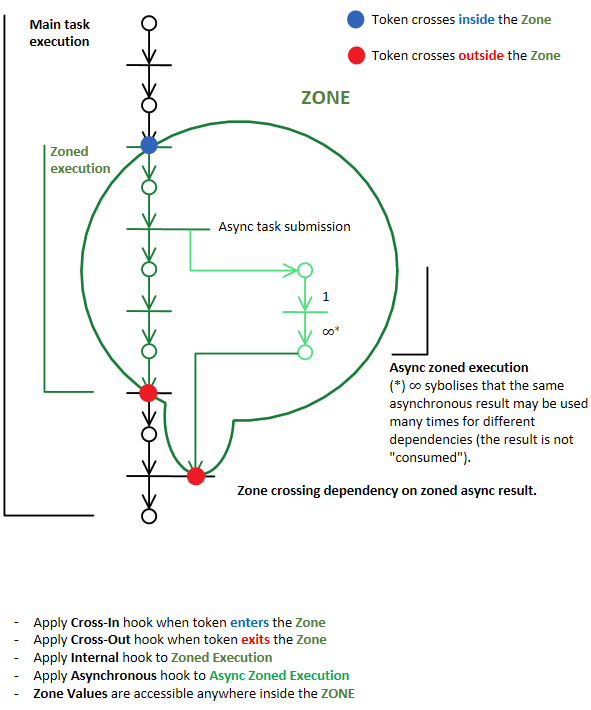
\includegraphics[width=\textwidth]{zone-pn}
  \caption{Zone on Petri net}
  \label{fig:zpn}
\end{figure}

More formally, given a Petri net $PN = (P, T, F)$ with $P$ the set of places, $T$ the set of transitions and $F$ the set of flows from $P$ to $T$ or $T$ to $P$: $F \subseteq (P \times T) \cup (T \times P)$, a Zone $Z$ is a subset $Z \subseteq P$ such that

$$\forall Z_1, Z_2 \exists Z_0 \text{ s.t. } Z_1 \subseteq Z_0 \land Z_2 \subseteq Z_0 $$

$$\forall Z_1, Z_2 (Z_1 \cap Z_2 \neq \emptyset) \Rightarrow [(Z_1 \subseteq Z_2) \lor (Z_2 \subseteq Z_1)] $$

Which more simply means: there exists a \emph{root} Zone enclosing all Zones and Zones can contain other Zones, but cannot intersect otherwise (figure \ref{fig:zinter}).

\begin{figure}[h]
  \centering
  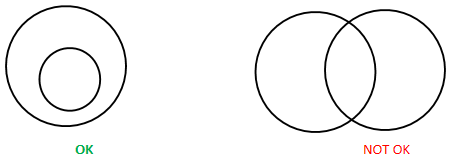
\includegraphics[width=\textwidth]{zone-intersect}
  \caption{Zone intersection}
  \label{fig:zinter}
\end{figure}

The key-value bindings defined by the Zone are accessible from any place inside that Zone. The crossing hooks are triggered whenever a token crosses a Zone boundary.

The Zone identifies a crossing event when a token of the Petri net moves between two places that do not belong to the same Zones (see crossing algorithm in section \ref{sec:cross-res}). For more liberty in the crossing hooks, tokens may carry nothing (void tokens) an error (error tokens) or the result of a zoned task (result tokens). In Java, the tokens are implemented as simple objects containing a result, an error value or nothing.

In order to know which Zone originated a token, they are wrapped as zoned tokens. A zoned token is simply a tuple containing a Token and its source Zone.

Operations on token while crossing Zone boundaries are described by the Zone's crossing hooks.
The presence of around hooks defined in the Zone allows even more capabilities. However, unlike the crossing hooks, these around hooks are closer to an implementation feature than a primary effect of the model.

\section{Terminology}

In order to ease further discussion and presentation of the Zone, this section gives a small glossary of the essential terms used in the Zone.


\paragraph{Task} represents the very general concept of ``something the program has to do''. More formally, a task is a procedure with some input and zero or one output. For example, \lstinline{Runnable} is a task with no input, no output. A method call is a task with method's arguments as input and method's return value as output.

\paragraph{Zoned Token} A zoned token is a tuple containing a token with its origin Zone. Zoned tokens are used as input to the cross resolution algorithm (see cross resolution section).

\paragraph{Zoned Task} A zoned Task is the result of binding a task to a Zone. A Zoned task behaves like a task but accepts and return only zoned tokens. For instance a task expressed in Java by
\begin{lstlisting}
Function<T, U> task;
\end{lstlisting}
Is associated to a zoned task represented by
\begin{lstlisting}
Function<ZonedToken<T>, ZonedToken<U>> zonedTask;
\end{lstlisting}

\paragraph{Zone Stack} is the stack of all enclosing zones at a given point of the program execution. Innermost Zone is considered to be at the top of the Zone Stack. If no Zone is defined, the current Zone is considered to be the default root Zone. For example :

\begin{lstlisting}
(new ZoneA()).run(() -> {
  /*
   * Zone stack here is:
   * ZoneA, ROOT_Zone
   */
   (new ZoneB()).run(() -> {
     /*
      * Zone stack here is:
      * ZoneB, ZoneA, ROOT_ZONE
      */
   });
});
/*
 * Zone stack here is back to:
 * ROOT_ZONE
 */
\end{lstlisting}

\section{Crossing Resolution}
\label{sec:cross-res}

The crossing principle is the original feature of the Zone. The base mechanism is simple. Value outputted by zoned tasks are \emph{zoned tokens}. When the value of a zoned token is used, it is extracted out of the zoned token to the current Zone, triggering the crossed Zones crossing hook.

Multiple cases can occur with the crossing mechanism. Especially in the Java implementation, where it is possible to keep and carry around references to already bound tasks, a token extraction can arise in unexpected contexts. Rather than relying on visibility restrictions to prevent such unusual cases to occur, the cross resolution properly defines how the model behaves under such circumstances.

For better understanding, keep in mind that at the bottom of every single Zone stack, there is the Root Zone. The Root Zone can be seen as the Zone with no hooks and values enclosing the whole program.

In the given code examples, \lstinline{new Zone()} creates a Zone whose parent is the enclosing Zone. For instance:

\begin{lstlisting}
Zone zone1 = new Zone();
Zone zone2;
zone1.run(() -> {
  // inside zone1
  zone2 = new Zone();
});

assert(zone1.getParent() == ROOT_ZONE);
assert(zone2.getParent() == zone1);
\end{lstlisting}

The cross resolution algorithm always receives three parameters :

\begin{enumerate}
\item The source Zone
\item The destination Zone
\item The crossing Token
\end{enumerate}

The crossing token is \emph{not} a zoned token. The zoned tokens used by the framework provide the source Zone of the cross resolution algorithm and the crossing token. The destination Zone is the current Zone of the extraction.

The crossing algorithm is divided in four steps:
\begin{enumerate}
\item Collect the Zone stack of the source Zone and the destination Zone to get the source stack and the destination stack.
\item Eliminate the common bottom part of the stacks. Recall that every Zone is a (indirect) child of the Root Zone, hence both stacks have at least one Zone in common. The idea of this step is to find the closest common enclosing the source and destination Zones: the \emph{join Zone}.
\item Cross out the rest of the source stack in top-down order with the crossing token. This means calling each crossing hooks of the crossed Zone with the crossing token as argument.
\item Cross-in the rest of the destination stack in down-top order with the crossing token.
\end{enumerate}

Let's see some concrete example of crossing executions.

\subsection*{Base case}

The common case of zoned execution is running code in a child Zone.

\begin{lstlisting}
// current Zone = some Zone

(new Zone()).run(() -> {
  // current Zone = new Zone

  // do zoned stuff here
});
\end{lstlisting}

When the code zoned in new Zone starts, the cross algorithm executes in a very simple configuration.

\begin{tabular}{| l | l |}
\hline
\textbf{Source Zone} & Some Zone
\\ \hline
\textbf{Destination Zone} & New Zone
\\ \hline
\textbf{Join Zone} & Some Zone
\\ \hline
\multicolumn{2}{l}{}
\\ \hline
\textbf{Source Zone Stack} & Some Zone :: ROOT\_ZONE
\\ \hline
\textbf{Destination Zone Stack } & New Zone :: Some Zone :: ROOT\_ZONE
\\ \hline
\textbf{Common Part} & Some Zone :: ROOT\_ZONE
\\ \hline
\multicolumn{2}{l}{}
\\ \hline
\textbf{Pruned Source Stack} & $\emptyset$
\\ \hline
\textbf{Pruned Destination } & New Zone
\\ \hline
\end{tabular}

Since the join Zone is the source Zone, the left source stack after step 2 is empty. Step 3 of the algorithm has no effect. No cross-out hook is applied, only one cross-in, of the destination Zone, is executed.

When the code zoned in new Zone ends, the cross algorithm executes in the dual configuration, still simple:

\begin{tabular}{| l | l |}
\hline
\textbf{Source Zone} & New Zone
\\ \hline
\textbf{Destination Zone} & Some Zone
\\ \hline
\textbf{Join Zone} & Some Zone
\\ \hline
\multicolumn{2}{l}{}
\\ \hline
\textbf{Source Zone Stack} &  New Zone :: Some Zone :: ROOT\_ZONE
\\ \hline
\textbf{Destination Zone Stack } & Some Zone :: ROOT\_ZONE
\\ \hline
\textbf{Common Part} & Some Zone :: ROOT\_ZONE
\\ \hline
\multicolumn{2}{l}{}
\\ \hline
\textbf{Pruned Source Stack} & New Zone
\\ \hline
\textbf{Pruned Destination } & $\emptyset$
\\ \hline
\end{tabular}

The join Zone is still the source Zone, but the left destination stack is emptied by step 2. Step 3 executes one cross out (from the source Zone), step 4 executes no cross In. To summarize, in this case, a cross in is executed when entering the new Zone, a cross out is executed when entering the old Zone. So far, so good.

\subsection*{Running in parent Zone from child Zone}

This is a simple case that allows to see that starting code execution in a Zone does not necessarily implies crossing in.

\begin{lstlisting}
// keeps reference to parent Zone
Zone parent = new Zone();

parent.run(() -> {
  // inside Zone parent
  Zone child = new Zone();
  child.run(() -> {
    // inside Zone child

    // this is the point of interest
    parent.run(() -> {
      // Zoned code here !!
    });
  });
});
\end{lstlisting}

When the code zoned in parent (at the point of interest) starts, the cross algorithm executes with the opposite configuration as the base case :

\begin{tabular}{| l | l |}
\hline
\textbf{Source Zone} & Child Zone
\\ \hline
\textbf{Destination Zone} & Parent Zone
\\ \hline
\textbf{Join Zone} & Parent Zone
\\ \hline
\end{tabular}

When entering the Zone, the argument pattern is the same as when ending in the base case. Hence one cross-out will be executed, no cross-in. Reversely, one cross-in and no cross-out is executed when ending in the Zone.
It is interesting to note that running in parent does not add layers on the Zone stack, but effectively pops the child Zone out of it. Adding once more the parent Zone on the Zone stack would not make sense, since the parent is an instantiation of a Zone, defining its own Zone stack (the context in which it was instantiated).


\subsection*{Entering a Sibling Zone}

This last example shows how, in one single crossing resolution, can both cross-in and cross-out hooks be triggered.

\begin{lstlisting}
(new Zone()).run(() -> {
  // inside parent Zone

  Zone child1 = new Zone();
  Zone child2 = new Zone();

  child1.run(() -> {
    // inside child1
    
    // this is the point of interest
    child2.run(() -> {
      // Zoned code here !!
    });
});
\end{lstlisting}

In this case, \lstinline{child1} and \lstinline{child2} share the same parent but neither is parent of the other one. Hence, when the code zoned in \lstinline{child2} (at the point of interest) starts, the cross resolution algorithm gets following configuration:

\begin{tabular}{| l | l |}
\hline
\textbf{Source Zone} & Child 1 Zone
\\ \hline
\textbf{Destination Zone} & Child 2 Zone
\\ \hline
\textbf{Join Zone} & Parent Zone
\\ \hline
\end{tabular}

Unlike previous cases, the join Zone is neither the source or the destination Zone. At the beginning of the zoned code, the step 3 triggers one cross-out from child 1, then the step 4 triggers one cross-in to child 2. As intended by the written code, at no point, parent Zone gets crossed in or out. The whole execution happens \emph{inside} the parent Zone.

\section{Task Binding}

This section presents how Zones and tasks interact. Specifically, what makes a task \emph{zoned} and how to bind a task to a Zone.

A zoned task has contextual access to the current Zone. At any point of its execution in a Zone, a task must be able to refer to that Zone. This reference gives
access to the Zone local values.

The context of a zoned task persists asynchronously. If an asynchronous task is started from a Zone, it must keep contextual access to that Zone.

Every element crossing a Zone boundary triggers its \emph{crossing hooks} (discussed in Cross Resolution section).

Code executed inside the Zone is intercepted and passed to its \emph{internal hooks}. The code that executes inside a Zone can be manipulated by the Zone itself, according to its hooks specification. Here is an illustration of an internal Zone execution:

\begin{lstlisting}
Zone myZone = ...

myZone.run(() -> {
  // code enclosed in this block is 'zoned' and
  // hooked as internal execution
  // by the 'internal hook' of myZone
});
\end{lstlisting}

In the same way internal execution is hooked, asynchronous submission in a zoned task is intercepted by the Zone.
Asynchronous submission inside a Zone can be manipulated by the Zone itself, according to its hooks content. This typically occur in this pattern:

\begin{lstlisting}
Zone myZone = ...

Executor myExecutor = ...

myZone.run(() -> {
  // inside myZone

  myExecutor.execute(() -> {
    // code enclosed here is still zoned in myZone and
    // hooked as asynchronous submission
    // by the 'async hook' of myZone
  });
  
});
\end{lstlisting}

\subsection*{Internal Binding}

The internal binding and execution of a task follow six steps :
\begin{enumerate}
\item Task is bound to the Zone, run hooks are applied.
\item The current Zone reference is updated to the Zone of execution.
\item An empty token crosses to the Zone of execution (Cross Resolution applied).
\item The task, hooked by the Zone, executes.
\item The current Zone reference is updated to the initial Zone (before task execution).
\item The result token crosses to the initial Zone (Cross Resolution applied).
\end{enumerate}

\subsection*{Asynchronous Binding}

The asynchronous binding and execution is quite different from the internal one. Unlike internally bound task, asynchronous task does not automatically trigger crossing operation. In fact, it is not possible a-priori to know when the task will be executed, from which context will come its input (if the task depends on the execution of another task) neither in which context will be used its output (if another task depends on the execution of this task). This summarizes to the following two points:
\begin{enumerate}
\item An asynchronously zoned task input may come from another Zone (hence causing crossing hook operations)
\item An asynchronously zoned task output may be used in another Zone (hence causing crossing hook operations)
\end{enumerate}

Since the crossing resolution is done on use-site, it takes into account its specific execution context :
\begin{enumerate}
\item An input coming from the same Zone does not trigger any cross operation.
\item An input coming from a parent Zone crosses inside the child Zone.
\item An input coming from a child Zone crosses outside the parent Zone.
\item An input coming from a sibling Zone (same parent) crosses outside the sibling Zone (towards the common parent Zone), then crosses inside the target Zone.
\end{enumerate}

This implements the intuition that a Zone encloses everything happening inside it and the cross operations are triggered if and only if something enters or exits the Zone.
For comparison with internal binding, asynchronous binding and execution of a task follow 6 steps:

\begin{enumerate}
\item Task is bound to the Zone, asynchronous hooks are applied. \\ \\
\textit{execution continues asynchronously...} \\
\item The current Zone reference is updated to the Zone of execution.
\item All inputs cross to the Zone of execution (crossing resolution applied once per input).
\item The task, previously modified by the Zone's asynchronous hook, executes.
\item The current Zone reference is updated to the initial Zone.
\item The result is returned in a zoned token, bound to the emitting Zone. The crossing resolution is not applied immediately but later, each time the zoned result gets used.

\end{enumerate}

\section{Properties} % TODO

The three aforementioned properties, crossing hooks, around hooks and Zone values are defined and used by the Zone as follows.

\subsection*{Zone Values}
Zone values storage implements Java-like block scoping rules: an inner Zone sees and can shadow its outer Zone values, but the opposite does not hold. Since Zone values are accessible from anywhere (especially from concurrent contexts), the Zone storage is immutable to limit the risk of race conditions. Note that, in Java, it is still possible to have an immutable reference to a mutable value to bypass this restriction.

The Zone allows to lookup a key for one value, but also to fully lookup a key to retrieve the list of all values defined for that key in each Zone of the Zone stack.

\subsection*{Crossing Hooks}

The crossing hooks are defined by the Zone as function from token to token. Note that in other code examples, the generic type parameter is omitted for the sake of simplicity.

\begin{lstlisting}
public <T> Token<T> crossIn(Token<T>);
public <T> Token<T> crossOut(Token<T>);
\end{lstlisting}

Hence, the crossing hooks can inspect the token, make computations and return a \emph{new} token with updated value. It is required that tokens are immutable. The reason is that the same zoned token may be used multiple times. If multiple tasks depend on the same asynchronous execution (hence having multiple callbacks for one method), its resulting token will be used once per dependency. Then it is crucial to always use the same unmodified token, not mentioning the risk of race conditions, if two concurrent crossing hooks run with the same zoned Token.

\subsection*{Around Hooks}

Around hook discussion distinguished the internal hooks and asynchronous hooks, but both make the same task. Only their application points differ. That is why they are not distinguished here and aggregated under the term of ``around hook''.

Around hooks are represented as function from zoned task to zoned task. Again, for simplicity, other code examples do not show the generic type parameters.

\begin{lstlisting}
public <T, U> ZonedTask<T, U> asyncHook(
        ZonedTask<T, U> zTask);
public <T, U> ZonedTask<T, U> internHook(
        ZonedTask<T, U> zTask);
\end{lstlisting}

This gives the opportunity to surround hooked task with a try-catch block, offers the choice  to execute or not the hooked task and even to run the task in a dynamically created Zone. Moreover, in a Zone, around hooks are inherited from enclosing Zones and applied from innermost to outermost hook~(figure~\ref{fig:around-hook}).

\begin{figure}[h]
  \centering
  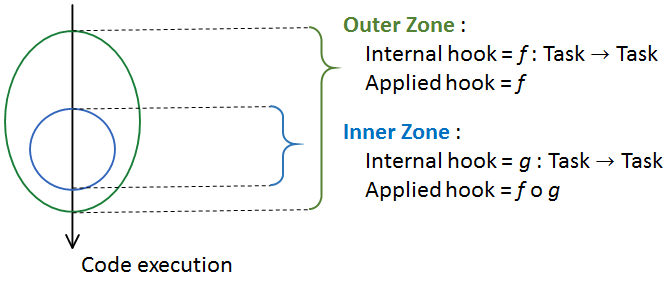
\includegraphics[width=0.7\textwidth]{around-hook}
  \caption{Around hook}
  \label{fig:around-hook}
\end{figure}

\subsection*{Around Hooks Inheritance}

For more flexibility, around hooks are inherited but not repeated. Consider three zones :

\begin{tabular}{|l|l|l|l|}
\hline
\textbf{Zone} & \textbf{Enclosing Zone} & \textbf{Defined hook} & \textbf{Applied hook}
\\\hline
outer Zone & None & $f$: Task $\rightarrow$ Task & $f$
\\\hline
middle Zone & outerZone & $g$: Task $\rightarrow$ Task & $f \circ g$
\\\hline
inner Zone & middleZone & $f$: Task $\rightarrow$ Task & $f \circ g$
\\\hline
\end{tabular}

In inner Zone, $f$ hook does not get applied one more time, because it would repeat inherited f hook from outer Zone. When the same hook is inherited multiple times, the outermost origin determines its application position. In the previous example, inner Zone applies $( f \circ g )$ and not $( g \circ f )$ because the outermost origin of $f$ (outer Zone) encloses the outermost origin of $g$ (middle Zone). This prevents inner Zones from accidentally modifying inherited hooks application order.

This inheritance policy is simply more general than a blind straight-forward application of all hooks. It is easy (especially in Java) to re-create a different instance of a hook with the same functionality to prevent it from being filtered out. On the other hand, given a single function composed of many hooks, it is hard, if not impossible, to filter out repetitions to get such union-inheritance.

\section{Realization}
\label{sec:realization}

The hypothesis that any submitted asynchronous code can be hooked permits to safely ignore the Zone integration when discussing its functionalities. The integration will be always possible. This is a great benefit, since it effectively decouples the Zone functional specification from its integration concerns, confronted to the multitude of evolving asynchronous frameworks in Java.

To integrate a Zone in a program, one can see it as a generalization of a Java thread local\footnote{A Java thread local is a field that is unique for each thread}. Note that the concept of thread local is not limited to Java. A mapping from threads to stored values easily implements a thread local behavior.

When using a thread pool, the concept of thread local becomes mitigated, even erroneous. Thread locals are bound to a specific thread, but the user does not controls how its tasks are bound to the threads. The common pattern to solve this is to wrap submitted code with instructions that update the thread local for the code.
\begin{lstlisting}

ThreadLocal<T> threadLocal = ...
Executor executor = ...

/*
 * Submitted code will update
 * the thread local on execution.
 */
public void submitWithLocal(Runnable code, T local) {
  Runnable newCode = () -> {
    // saves initial value
    T initial = threadLocal.get();

    // sets desired value for code
    threadLocal.set(local);
    code.run();

    // restores initial value
    threadLocal.set(initial);
  };

  executor.execute(newCode);
}
\end{lstlisting}

The Zone is a generalization of this method. Rather than binding a runnable, any code is accepted, denoted as \emph{task}. The Zone handles internally the thread local to store itself and simply exports a bind method.
The Zone takes advantage of this binding operation to apply its internal mechanics and all defined submission hooks. Based on this single binding, it provides:
\begin{itemize}
\item Asynchronous persistent context.
\item Modeled execution flow between the Zones.
\item Flexible programmable hooks on Zone transitions and code submission to the Zone.
\item Extension and reusability mechanisms to extend and implement more Zone features.
\end{itemize}


This pattern efficiently decouples the Zone integration from its functionalities. To use it, one only needs to bind each submitted asynchronous task to the Zone. This can be even simpler using a ``Zone-aware executor'' (see chapter \ref{ch:inpractice} for an example).

Chapter \ref{ch:asyncworld} showed that in Java, one cannot assume a single execution framework. The presented binding solution is not a uniform solution that automagically works in any context. It describes a single operation to execute on every asynchronous submission, which can even be modularized in the execution framework. That is how the Zone gets integrated in programs.


\chapter{Existing Approaches}
\label{ch:approaches}

The Zone exists already for Dart and JavaScript. Those frameworks were the inspiration of asynchronous execution context for the Java Zone. Both \zonejs\ and \zonedrt\ define Zone local storage, execution hooks (in the sense of around hook for the Java Zone) and error handling. The error handling includes for both long stack trace generation. \zonejs\ implements the sytematic error handling for its call-back centered structure. \zonedrt\ follows the contextual error handling in its future-based approach.

\begin{figure}[h]
\centering
\begin{tabular}{| p{0.3\textwidth} | p{0.19\textwidth}  | m{0.19\textwidth} | m{0.2\textwidth} |}
\hline
 & \textbf{\zonejs} & \textbf{\zonedrt} & \textbf{Java Zone}
\\\hline
\textbf{Multi threaded} & no & no & yes
\\\hline
\textbf{Zone local storage} & yes & yes & yes
\\\hline
\textbf{Distinction internal-asynchronous hook} & yes & no & yes
\\\hline
\textbf{\emph{Around} hooks} & no & yes & yes
\\\hline
\textbf{Extensible API} & no & no & yes
\\\hline
\textbf{Before, Return, After hooks} & yes & no & plugin 
\\\hline
\textbf{Long stack trace} & yes & yes & plugin
\\\hline
\textbf{Promises support} & no & yes & plugin
\\\hline
\textbf{Crossing mechanism} & no & no & yes
\\\hline
\textbf{Out of the box basic tools} & yes & yes & no
\\\hline
\textbf{Adaptable to multiple frameworks} & no & no & no
\\\hline
\end{tabular}
\caption{\zonejs, \zonedrt\ and Java Zone comparison}
\label{fig:zcomp}
\end{figure}


In comparison to \zonejs\ and \zonedrt, the Zone for Java archives greater generality and, in my honest opinion, better founded execution principle. The Zone model gives arguments and a representation to understand how the Java Zone works, by opposition to \zonejs\ and \zonedrt\ who just implement usecases in answer to concrete problems.

Of course, this level of abstraction comes at the cost of increased complexity. For example, to get a long stack trace, one has to make a decision of how he will implement his asynchronous error handling, contextual or systematic~? Then based on his decision, he chooses the correct hooks to add the asynchronous call stack of the Zone into handled errors.

There is an emerging project, driven by StrongLoop, to provide a Zone in the Node.js environment. However it is not an adaptation of \zonejs\ but a new implementation of the Zone, specific for Node.js. In the equivalent situation (see chapter \ref{ch:inpractice}, the integration of the Java Zone into \vertx was almost transparent and required only to develop adaptor code. No Zone functionality were rewritten and all existing specified Zone implementations are directly reusable.

This adaptability of the Java Zone, and its high composability are the main benefits brought by the Java Zone over \zonejs\ and \zonedrt.


\chapter{Practical Experiments}
\label{ch:inpractice}

This chapter shows two experiments and their results of an advanced use of the Zone. The first realizes an asynchronous sequence diagram of a parallel program with dependencies. The second describe how to transparently instrument the third-party framework \vertx\ to realize a ``Zone-aware \vertx''.

\section{Asynchronous Sequence Diagram}


\paragraph{Specifying} what is interesting in an asynchronous sequence diagram is the most complex part if this experiment. In fact, producing the information of a conventional sequence diagram is not interesting. There are already many tools to do that. The useful data is an asynchronous dependency diagram: what are the dependencies between asynchronous tasks. The produced diagram is defined by:

\begin{itemize}
\item Each task execution is divided into sub parts, represented by the nodes of a graph.
\item Tasks are divided into the biggest possible parts such that a sub-part execution first uniquely shows \emph{incoming} dependencies (rely on other tasks result or completion). Then it uniquely shows \emph{outgoing} dependencies (another task shows incoming dependency from this task).
\item Dependencies are represented as directed edges between the corresponding nodes of their tasks.
\end{itemize}

The produced graph is a directed acyclic graph where each node represents an autonomous part of the programs and the edges show the precedences between those parts.

\paragraph{The realization} is then pretty easy using the Zone. As evoked in chapter \ref{ch:apps}, use the one Zone per task pattern, creating \lstinline{TaskZone}s. Each \lstinline{TaskZone} stores a unique task ID and defines the crossing hook: 

\begin{lstlisting}
// The cross operation executes inside -destination- Zone

// The cross operation is defined inside -source- Zone

public Token crossOut(Token token) {
  TaskZone sourceZone = this;
  int sourceID = sourceZone.taskId;

  int destID = Zone.lookup(TASK_ID_KEY);

  storeDependency(souceID, destID);
}
\end{lstlisting}

The difficult part is then to compile collected information and build a graphical representation. For the code of a fork-join algorithm (figure \ref{fig:fj-alg}) I used a sample code from the d3.js library to produce the view shown in figure \ref{fig:fjt-bundle}. Each node is named 'X\#Y'. 'X' is the task id and 'Y' the subtask id. The initial task is '0', split in two subtasks '0\#1' entry point of algorithm and '0\#2', end of the algorithm with output value.

\begin{figure}[h]
  \textbf{Solving problem $P$}
  \begin{enumerate}
  \item If $P$ is small then solve $P$.
  \item Else split $P$ in a list $P$s of smaller problems $p$.
  \item For each $p$ in $P$s, start an asynchronous task to solve $p$.
  \item Join each asynchronous task started in (3) and collect all sub-results.
  \item Compose the sub-results and return the final solution.
  \end{enumerate}
\caption{Generic fork-join algorithm}
\label{fig:fj-alg}
\end{figure}

\begin{figure}
  \centering
  \makebox[\textwidth][c]{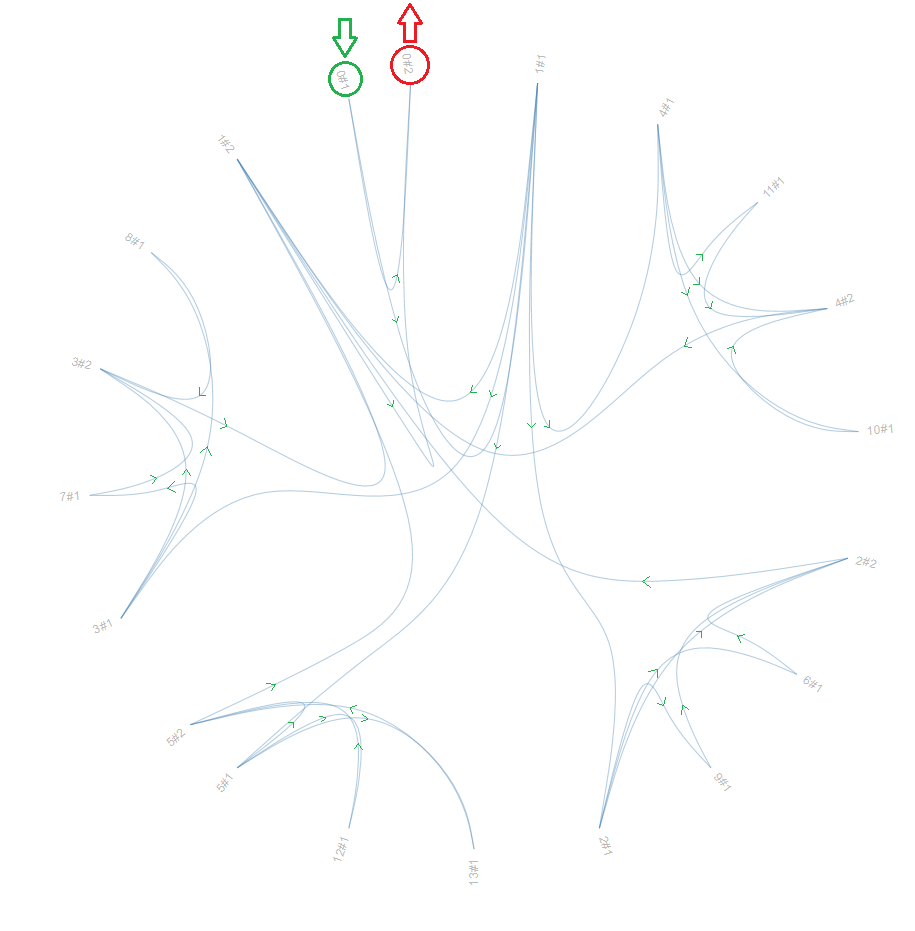
\includegraphics[width=1.4\textwidth]{bundle-fjt}}
  \caption{Fork-join algorithm dependency graph}
  \label{fig:fjt-bundle}
\end{figure}


\section{Transparent Instrumentation}

In this experiment, I used the AOP framework AspectJ to automatically instrument the \vertx\ library. If analyzing the \vertx\ code to define where and how to apply the Zone was tedious, the concrete realization was much simpler.

\paragraph{Results} of this work are:
\begin{itemize}
\item Integration code is quite small (only six classes of 60 lines in average).
\item Aspect weaving only relies on public \vertx\ API and assumes no internal behavior.
\item The instrumentation is done by a stand-alone program that produce an artifact interchangeable with the original \vertx.
\end{itemize}

``Interchangeable'' here means one can transparently be replaced by the other. If used on an existing project, the only thing to modify is the import resolution in the project configuration. Since the instrumented \vertx\ library completely reproduces the original package structure, the imports in the different classes do not need modification.

With this instrumented library, I was even able to reuse the classes developed for the asynchronous dependency diagram to visualize the dependencies of a \vertx\ program.




\chapter{Zone your Java}
\label{ch:impl}

This chapter closes the Zone presentation with a brief overview of its implementation and usage.
The aim is to give you an insight on the Zone architecture and get you familiarized with some utilization tips and tricks.

\section{Idioms}

Here is a small digressions about common used code patterns that may trouble a regular Java developer using the Zone.



\begin{itemize}
\item $\lambda$s typing and creation (especially for hooks)
\item Key-typed-map and Heap pollution concerns
\item The match function (use Option class for Zone values lookup)
\end{itemize}

\section{Make your Zone}

\begin{itemize}
\item Zone class extension - implement your hooks
  \begin{itemize}
  \item cross in - out method
  \item get around hooks (sync and async) method
  \item get value method
  \end{itemize}
\item Use embedded zone (value zone, around zone, b-r-a zone, cross zone, error zone)
\item Build your own zone property (as in last point of application)
\end{itemize}


\section{Zoned Executors}

As evoked in (some previous chapter), the Zone integrates on top of an asynchronous execution framework. In order to make zone fully functional (regarding asynchronous invocations), you will need either

Use an instrumented execution framework :
\begin{itemize}
\item Executor, ExecutorService, CompletableFuture (with limitations of replacing JRE classes by others : different packages/naming
\item instrumented third part library, \vertx\ example.
\end{itemize}

Or instrument your own execution framework :
\begin{itemize}
\item Think to bind to Zone when user submits code to your API (which class stores executable code), not later, even if the . The user will expect
\item Be aware that if your API methods rely on other API method (overloaded method to provide default argument), you should not bind submitted code twice.
\item If your framework rely only on another executor (i.e. does not store any form of executable code), you can simply bind any code submitted to that executor, or better, use a zone-instrumented version of that executor.
\item Think Zoned. As long as you don't make an asynchronous execution, context is automatically preserved (same thread)
\item Be aware of race conditions. Zones are shared among concurrent parts of programs by nature + crossing hooks \emph{will} execute in foreign Zone : An object modified by a crossing hook is not Thread safe, even it is in a thread confined zone.
\end{itemize}

\chapter{Conclusion}
\label{ch:conclusion}

We have seen that the Zone for Java brings you innovative building tools. The integration work may be a little complex (as showed the \vertx\ case study), but once this is correctly done, one can almost transparently rely on the Zone as a uniform execution context. In summary, the Zone needs:
\begin{itemize}
\item Explicit binding to asynchronous tasks submitted to the framework.
\end{itemize}

In return, it brings:
\begin{itemize}
\item Persistent context over asynchronous transitions.
\item Modeled execution flow between Zones.
\item Flexible programmatic hooks on:
  \begin{itemize}
  \item Zone binding and execution.
  \item Asynchronous submission and execution.
  \item Execution flow across different Zones.
  \end{itemize}
\item Extensible and reusable structure.
\end{itemize}

To close this work, I'll show three ways of research and development on the Zone and a small analysis of how the original problematic changed through the research.

\section{Development}

Bringing more and easier binding primitives would be very interesting. Even though the binding principle is detailed, its implementation is still not general. This is mainly due to the large amount of standard interfaces present in the \lstinline{java.util.function} package that match to the Zone's task abstraction. Actually, the Zone only handles \lstinline{BiFunction} and requires additional wrap-steps to bind another interface, as \lstinline{Runnable} for example.

When using and probing the Zone, I often encountered the need to ignore parts of the Zone stack, or even to reorder the stack. Reordering would be useful to ensure some hook is always applied in first position. The union-inheritance is the solution I used to gain the required flexibility. However, nothing proves this is the only solution. 

The scope projection is one solution to theorize and specify the Zone stack manipulation. It consists in using a predicate on the Zone to filter the Zone stack, allowing to project the Zone context to another with only the properties of accepted Zones. One concrete use is to deduce a new context, based on the current one. This grants an easy way to keep some useful information and drop the data we don't use any more.

\section{Theory}

The representation on Petri nets is useful for understanding but not totally formalized. A strict theorizing will allow to relate, compare and even associate the Zone to existing Petri nets extensions. For example, colored Petri nets which store data inside its toke shares this particularity with the Zone. If such association exists, the Zone could benefit of existing results and asynchronous theorems, hence increasing its stability and the understanding we have of the Zone.

\section{Practice}

The zone stays a complex abstraction, especially realizing an integration on an execution framework is hard. A good improvement is to collect experience data and compile it as a best practices guide or a trouble shooting documentation. This can even lead to reworking some aspects of the model that would appear unsound.

An additional performance analysis will help to understand the cost of using the Zone. Indeed, it currently adds a lot of wrapping overhead. Knowing that overhead and bottlenecks of the framework opens the door to efficient optimization and determines if it suits to a production environment.



\section{Asynchronous problematic}

It was interesting to see how the central problematic evolved in the course of the development. At first, I was focused on creating a working implementation with hooks, with error handling, with values, and all other requirements to solve the asynchronous problems. Quickly, I realized that I was only treating the symptoms of the problem and started to look for analogies of all these different solutions. Is there an essential problem and a unique solution, on which all other specific properties can be realized?

Trying to answer that question, I found out that the real need is a \emph{uniform execution principle}, constant in both synchronous and asynchronous transitions. This gave birth to the crossing principle that I successfully used to implement specialized abilities on the Zone.

With these words, we can conclude that the real need to correctly deal with the asynchronous programming is not an overpowered framework with lots of features and incredible refinement to distinguish addressed cases. The real point is to find a simple representation to think about synchronous and asynchronous executions in a \emph{uniform} way.



%\appendix
\chapter{An appendix}







\end{document}

